\section{Evaluation}
\label{sec:eval}
\subsection{Experimental Settings}
\subsubsection{Datasets}
We built our blood glucose dataset from July 2016 to January 2017. A total of 112 users joined in our experiments. Table~\ref{dataset} illustrates the details of the dataset.
\begin{itemize}
  \item Blood Glucose Data: During the experiments, each user wears a CGM device to collect the blood glucose sample every 3 minutes. \sysname divides the blood glucose value into four levels by preset thresholds. The numbers of blood glucose samples in each level are shown in Table~\ref{dataset}. In our experiments, all the users are promise to wear CGM for at least 5 days. The distribution of experimental durations are listed in Table~\ref{dataset}.
  \item External Factors Data: In the duration of wearing the CGM, each user installs \sysname on smartphone to sense the daily activities and sleep quality automatically. Meanwhile, users also leverage \sysname to record their daily meals, drug and insulin input. \sysname transfers the external factors as variables of physiological model at corresponding time.
  \item User Basic Information Data: The users are required to record the basic personal data relevant to blood glucose (e.g., age, weight, gender and health status) into \sysname, which are listed in Table~\ref{dataset}. \sysname classifies the users into three groups based on their health status.

\end{itemize}





\begin{table}[]
\centering
\caption{The Details of Dataset}
\label{dataset}
\begin{tabular}{clccclcccccl}
\hline\hline
\multicolumn{12}{c}{\textbf{Blood Glucose}}                                                                                                                                                                                               \\ \hline
\multicolumn{2}{l}{\textbf{\cellcolor[gray]{0.8}Blood Level}} & \multicolumn{2}{r}{\textbf{\cellcolor[gray]{0.8}Level 1}} & \multicolumn{2}{c}{\textbf{\cellcolor[gray]{0.8}Level 2}} & \multicolumn{2}{c}{\textbf{\cellcolor[gray]{0.8}Level 3}} & \multicolumn{2}{c}{\textbf{\cellcolor[gray]{0.8}Level 4}} & \multicolumn{2}{c}{\textbf{\cellcolor[gray]{0.8}Total}} \\
\multicolumn{2}{l}{Number of Sample}     & \multicolumn{2}{c}{75369}            & \multicolumn{2}{c}{293530}           & \multicolumn{2}{c}{235686}           & \multicolumn{2}{c}{158054}           & \multicolumn{2}{c}{762639}         \\ \hline\hline
\multicolumn{12}{c}{\textbf{Experimental Duration}}                                                                                                                                                                                          \\ \hline
\multicolumn{2}{l}{\textbf{\cellcolor[gray]{0.8}Days}}        & \multicolumn{2}{c}{\textbf{\cellcolor[gray]{0.8}6-10}}    & \multicolumn{2}{c}{\textbf{\cellcolor[gray]{0.8}11-15}}   & \multicolumn{2}{c}{\textbf{\cellcolor[gray]{0.8}16-20}}   & \multicolumn{2}{c}{\textbf{\cellcolor[gray]{0.8}21-25}}   & \multicolumn{2}{c}{\textbf{\cellcolor[gray]{0.8}26-30}} \\
\multicolumn{2}{l}{Number of Users}      & \multicolumn{2}{c}{48}               & \multicolumn{2}{c}{24}               & \multicolumn{2}{c}{20}               & \multicolumn{2}{c}{13}               & \multicolumn{2}{c}{7}              \\ \hline\hline
\multicolumn{12}{c}{\textbf{User Basic Information}}                                                                                                                                                                                      \\ \hline
\multicolumn{2}{l}{\textbf{\cellcolor[gray]{0.8}Age}}         & \multicolumn{2}{c}{\textbf{\cellcolor[gray]{0.8}15-24}}   & \multicolumn{2}{c}{\textbf{\cellcolor[gray]{0.8}25-34}}   & \multicolumn{2}{c}{\textbf{\cellcolor[gray]{0.8}35-44}}   & \multicolumn{2}{c}{\textbf{\cellcolor[gray]{0.8}45-54}}   & \multicolumn{2}{c}{\textbf{\cellcolor[gray]{0.8}55-70}} \\
\multicolumn{2}{l}{Number of Users}      & \multicolumn{2}{c}{8}                & \multicolumn{2}{c}{17}               & \multicolumn{2}{c}{24}               & \multicolumn{2}{c}{29}               & \multicolumn{2}{c}{34}             \\
\multicolumn{2}{l}{\textbf{\cellcolor[gray]{0.8}Weight}}      & \multicolumn{2}{c}{\textbf{\cellcolor[gray]{0.8}30-44}}   & \multicolumn{2}{c}{\textbf{\cellcolor[gray]{0.8}45-54}}   & \multicolumn{2}{c}{\textbf{\cellcolor[gray]{0.8}55-64}}   & \multicolumn{2}{c}{\textbf{\cellcolor[gray]{0.8}65-74}}   & \multicolumn{2}{c}{\textbf{\cellcolor[gray]{0.8}75-90}} \\
\multicolumn{2}{l}{Number of Users}      & \multicolumn{2}{c}{18}               & \multicolumn{2}{c}{21}               & \multicolumn{2}{c}{32}               & \multicolumn{2}{c}{22}               & \multicolumn{2}{c}{19}             \\
\multicolumn{4}{l}{\textbf{\cellcolor[gray]{0.8}Gender}}      & \multicolumn{3}{c}{\textbf{\cellcolor[gray]{0.8}Male}}                                                               & \multicolumn{5}{c}{\textbf{\cellcolor[gray]{0.8}Female}}                                                          \\
\multicolumn{4}{l}{Number of Users}      & \multicolumn{3}{c}{57}                                                                          & \multicolumn{5}{c}{55}                                                                       \\ \hline\hline
\multicolumn{12}{c}{\textbf{User Health Status}}                                                                                                                                                                                          \\ \hline
\multicolumn{3}{l}{\textbf{\cellcolor[gray]{0.8}Health Status}}                   & \multicolumn{3}{c}{\textbf{\cellcolor[gray]{0.8}Health}}                     & \multicolumn{3}{c}{\textbf{\cellcolor[gray]{0.8}Type I}}                      & \multicolumn{3}{c}{\textbf{\cellcolor[gray]{0.8}Type II}}                  \\
\multicolumn{3}{l}{Number of Users}                          & \multicolumn{3}{c}{35}                                  & \multicolumn{3}{c}{38}                                   & \multicolumn{3}{c}{39}                                \\ \hline
\end{tabular}
\end{table}



\subsubsection{Ground Truth and Metrics}

The blood glucose samples collected by the CGM are regarded as groundtruth. We compare the prediction results of \sysname with the groundtruth, and the performance is measured in terms of the precision \cite{}, recall\cite{} and accuracy\cite{}.






%
%
%\begin{table}[]
%\centering
%\caption{The details of dataset}
%\label{The details of dataset}
%\begin{tabular}{|l|c|c|c|c|l|}
%\hline
%\textbf{Blood Level}                  & \textbf{Level 1} & \textbf{Level 2} & \textbf{level 3} & \textbf{Level 4} & \textbf{Total}         \\ \hline
%\multicolumn{1}{|c|}{\textbf{Number}} & 75369            & 293530           & 235686           & 158054           & \multicolumn{1}{c|}{762639} \\ \hline
%\end{tabular}
%\end{table}















\begin{table}[]
\centering
\caption{Confusion matrix of \sysname performance}
\label{tab:confusion_matrix}
\begin{tabular}{|c|c|c|c|c|l|l|}
\hline
\multirow{2}{*}{\textbf{\begin{tabular}[c]{@{}c@{}}Ground\\ Truth\end{tabular}}} & \multicolumn{4}{c|}{\textbf{Predictions}}                                                                                 & \multicolumn{2}{l|}{\multirow{2}{*}{}}                                                            \\ \cline{2-5}
                                                                                 & Level 1                      & Level 2                      & Level 3                      & Level 4                      & \multicolumn{2}{l|}{}                                                                             \\ \hline
Level 1                                                                          & \cellcolor[gray]{0.8}62657                        & 5521                         & 3672                         & 3519                         & 83.13\%                             & \multirow{4}{*}{\rotatebox{90}{\textbf{Recall}} }                           \\ \cline{1-6}
Level 2                                                                          & 16346                        &  \cellcolor[gray]{0.8}240584                       & 27563                        & 9037                         & 81.96\%                             &                                                             \\ \cline{1-6}
Level 3                                                                          & 2660                         & 30905                        & \cellcolor[gray]{0.8}188472                       & 13649                        & 79.97\%                             &                                                             \\ \cline{1-6}
Level 4                                                                          & 3443                         & 5620                         & 14278                        & \cellcolor[gray]{0.8}134713                       & 85.23\%                             &                                                             \\ \hline
\multicolumn{1}{|l|}{\multirow{2}{*}{}}                                          & \multicolumn{1}{l|}{73.62\%} & \multicolumn{1}{l|}{85.12\%} & \multicolumn{1}{l|}{80.55\%} & \multicolumn{1}{l|}{83.72\%} & \multicolumn{2}{l|}{\multirow{2}{*}{\begin{tabular}[c]{@{}l@{}}Accuracy:\\ 82.14\%\end{tabular}}} \\ \cline{2-5}
\multicolumn{1}{|l|}{}                                                           & \multicolumn{4}{c|}{\textbf{Precision}}                                                                                 & \multicolumn{2}{l|}{}                                                                             \\ \hline
\end{tabular}
\end{table}



\subsubsection{System Evaluation}

To evaluate the \sysname performance, we provide CGM for each new user for one time usage, supporting more than 5 days. We take the former 4 days as the training data, and left days as the testing data. If the left days of one users are longer than 2 days, we calculate the user's average performance. Table~\ref{tab:confusion_matrix} shows the results of testing dataset. As we can see,  the recalls of four blood glucose levels are above 79\%, and all the precisions of four blood glucose levels keep above 73\%. In particular, the recalls of level 1 and level 3 are 83.13\% and 85.23\%, demonstrating the high sensitivity of \sysname towards these two levels. The 82.14\% accuracy states the outstanding prediction performance of \sysname.


\subsubsection{Evaluation on Multi-task Model structure}
To demonstrate the effectiveness of \modelname structure, we compared our model over the following combinations.

\begin{itemize}

  \item \emph{General Learning}:
  All the users shared a same information representation, dynamic and personality layers, which assumes the blood glucose trends of all users can be tracked by a same model.


  \item \emph{Single Learning }:
  Each user is trained for a specific model.

  Fig.~\ref{fig:cmp_model} shows the results.
\end{itemize}


\begin{figure}[!t]
\centering
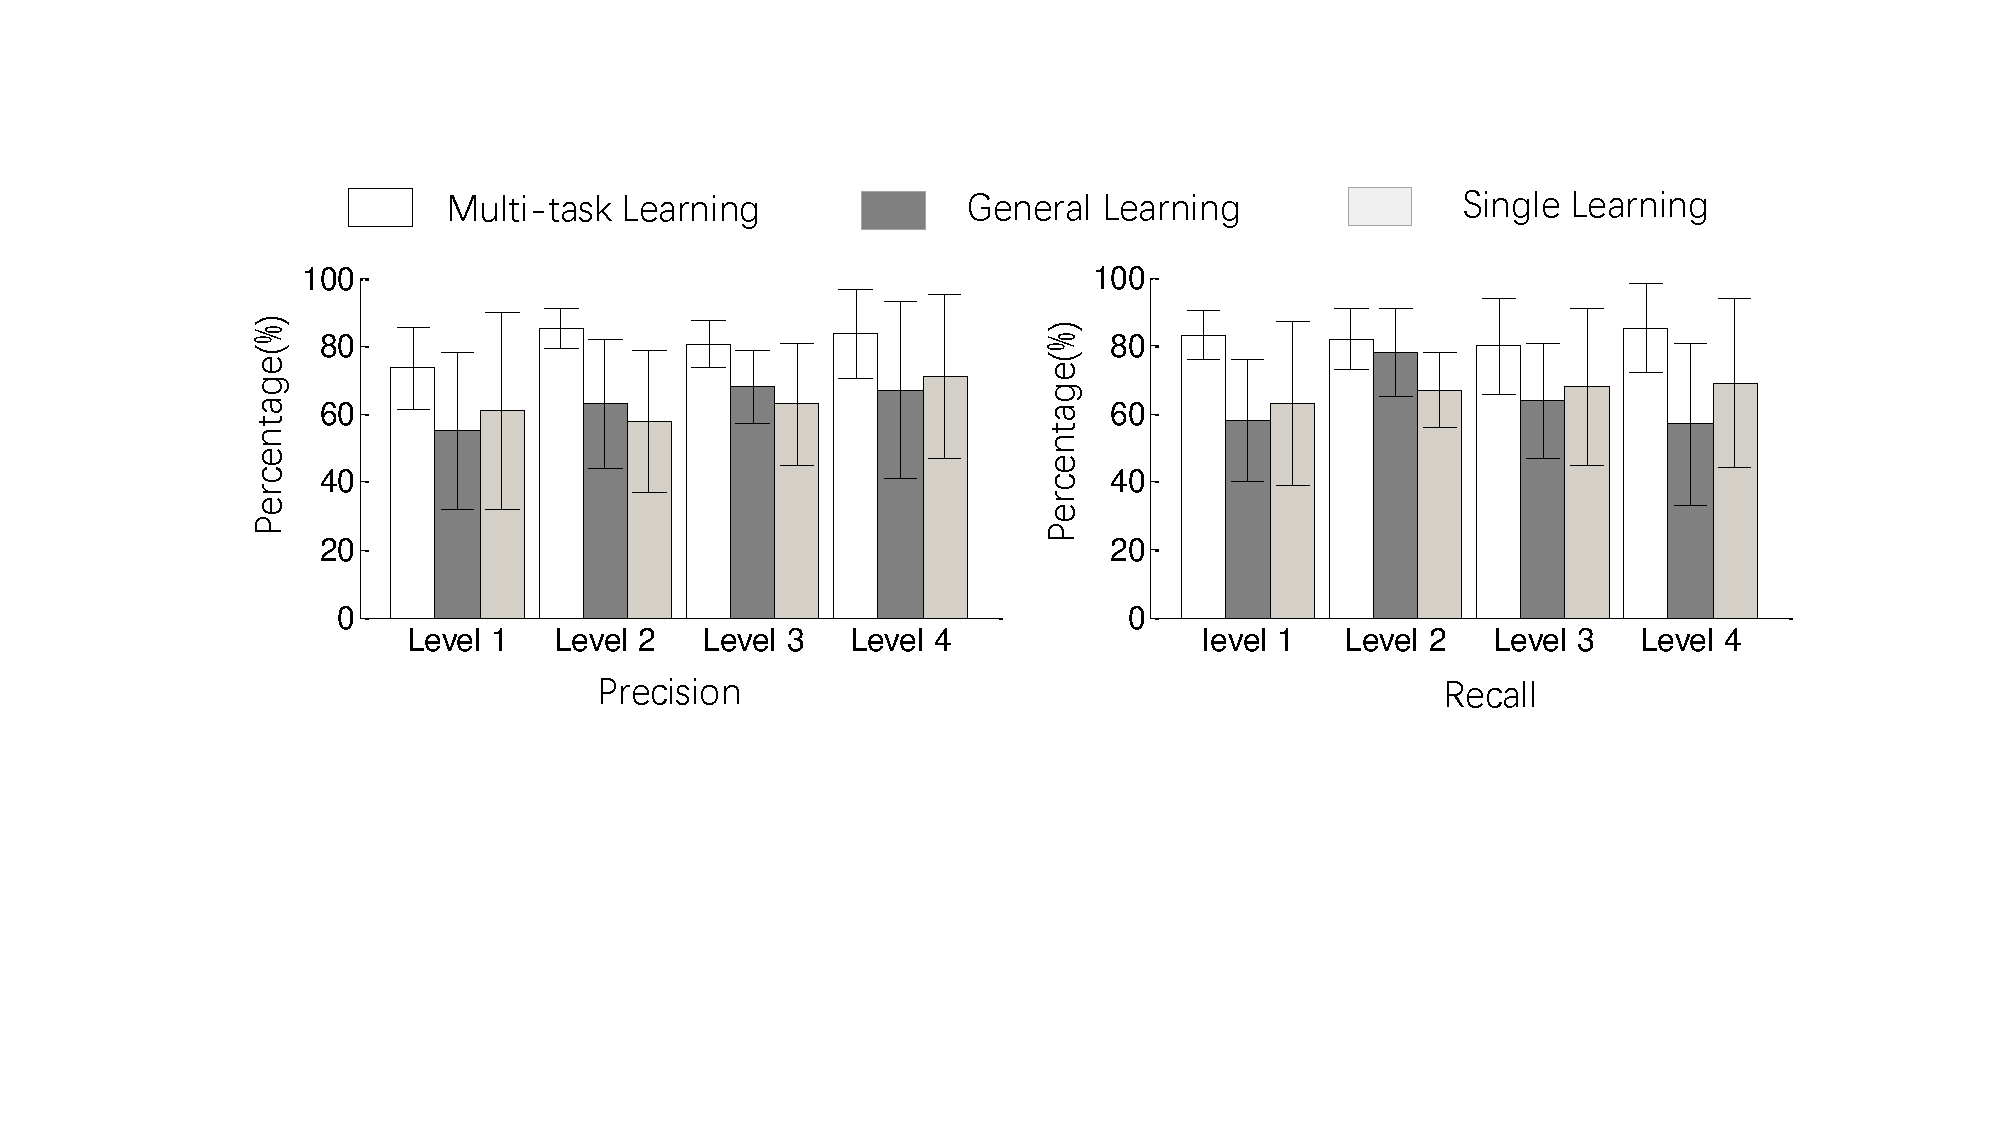
\includegraphics[width=0.9\columnwidth]{./img/CMP_Models.pdf}
\caption{The model comparison}
\label{fig:cmp_model}
\end{figure}


\subsubsection{Multi-task Model and General Model Comparison in Group}
We also apply general learning approach on the users in same group, and compare the prediction performance of \modelname. Fig.~\ref{fig:cmp_groups}
shows the results. As is shown, \modelname outperforms the general learning methods in each group, especially the performance of level 1 and level 4. It mainly results by two reasons. On the one hand, the limitation of blood glucose data in each group weakens the capability of temporal dynamic characteristics. On the other hand, the imbalanced distribution of blood glucose data of one group also low the performance down. For example, much more data of level 4 and much less data of level 1 in group 3 (type II diabetes) low down the recall of level 1 and the precision of level 4. It is even hard to be solved by the cost sensitive approach.


\begin{figure}[!t]
\centering
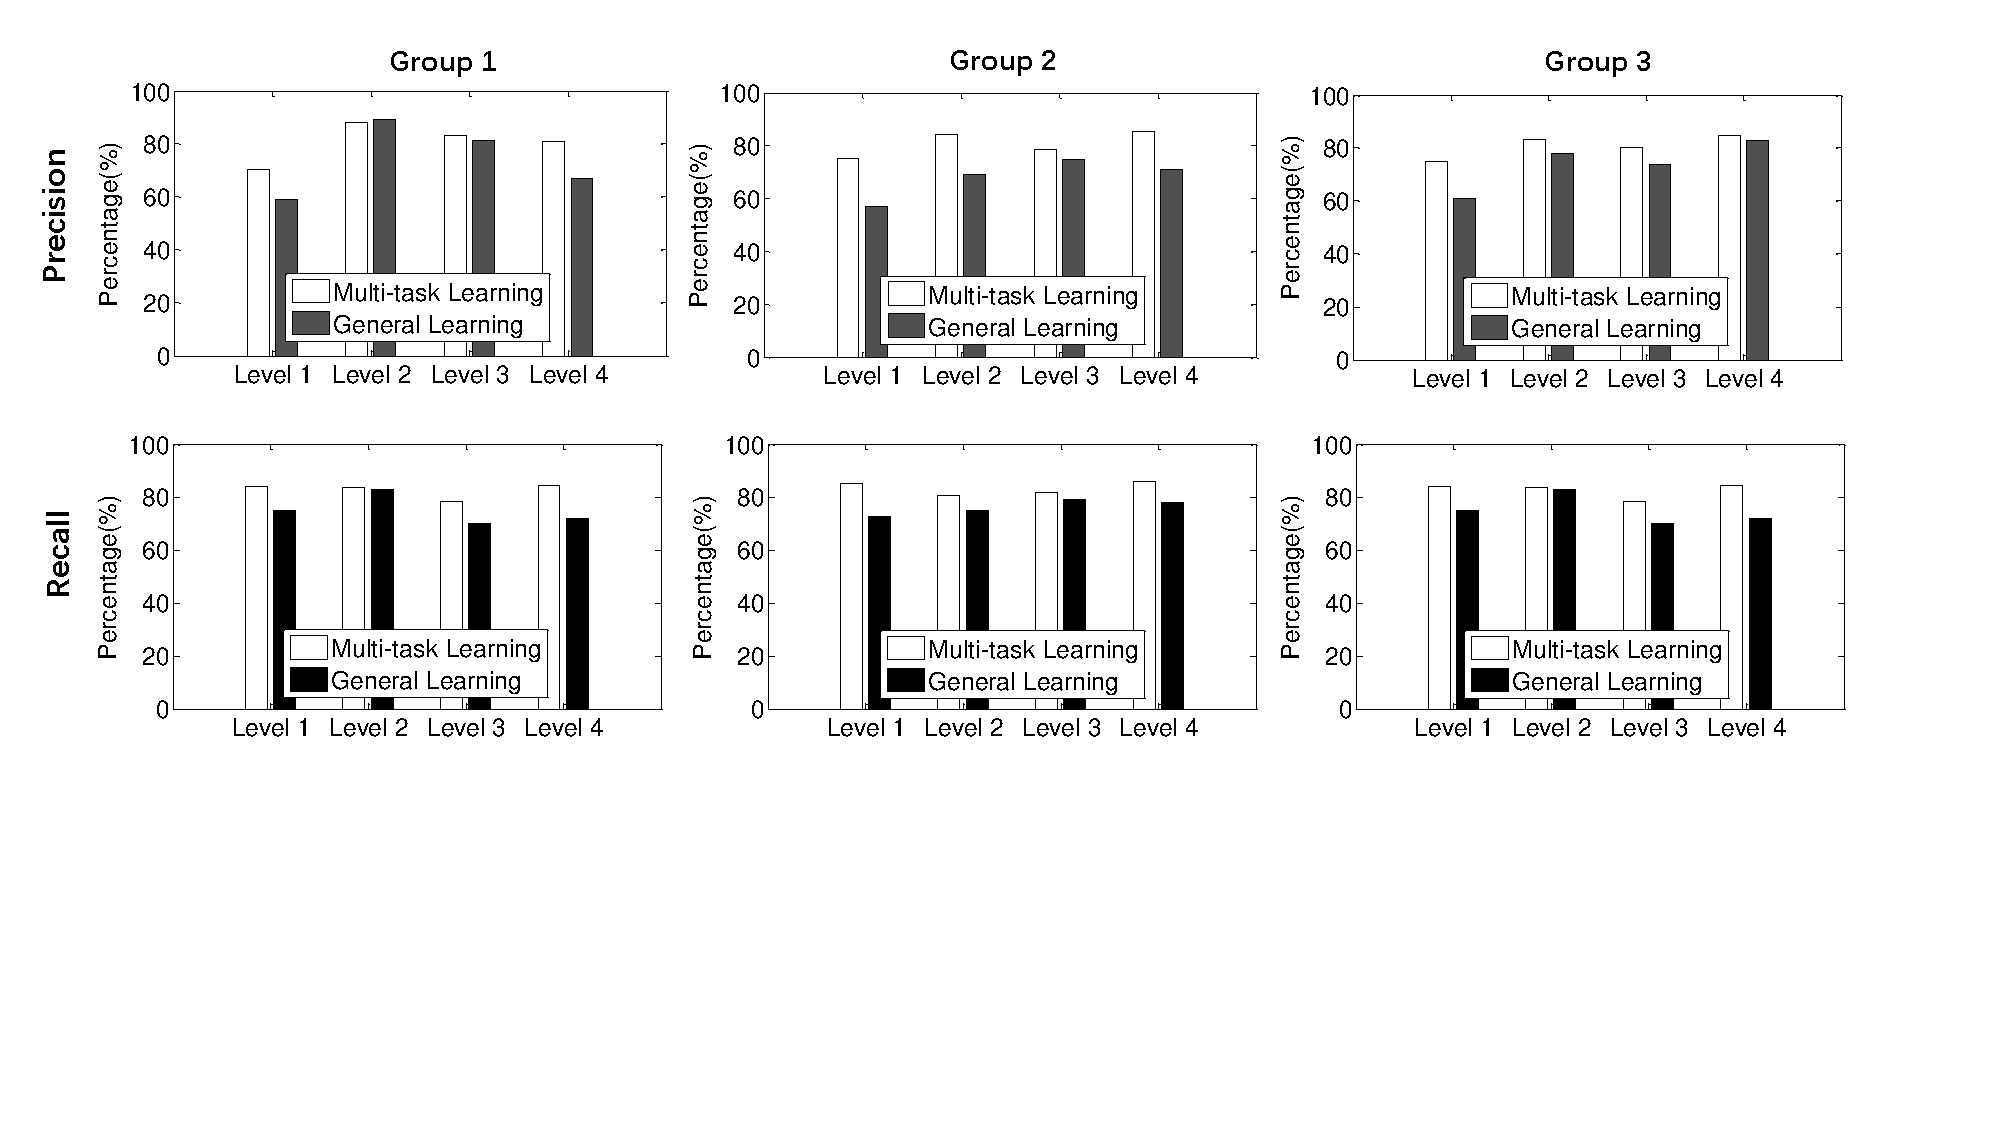
\includegraphics[width=0.9\columnwidth]{./img/group_multi_task.pdf}
\caption{The comparison of multi-task learning and group general learning.}
\label{fig:cmp_groups}
\end{figure}


\subsubsection{Evaluation with various training data}

Since the users may wear CGM continuously, we evaluate the performance of \sysname with increasement of training dataset by five days. Under each system evaluation, we trained all the data of the users with before the testing date, and measured the system by calculating the average performance of those who have longer testing days.

Fig.~\ref{fig:per_under_train_days} illustrates the results. We can see the system performance grow up with the increasement of training dataset, demonstrating the performance of \sysname will grow up with more training data.


\begin{figure}[!t]
\centering
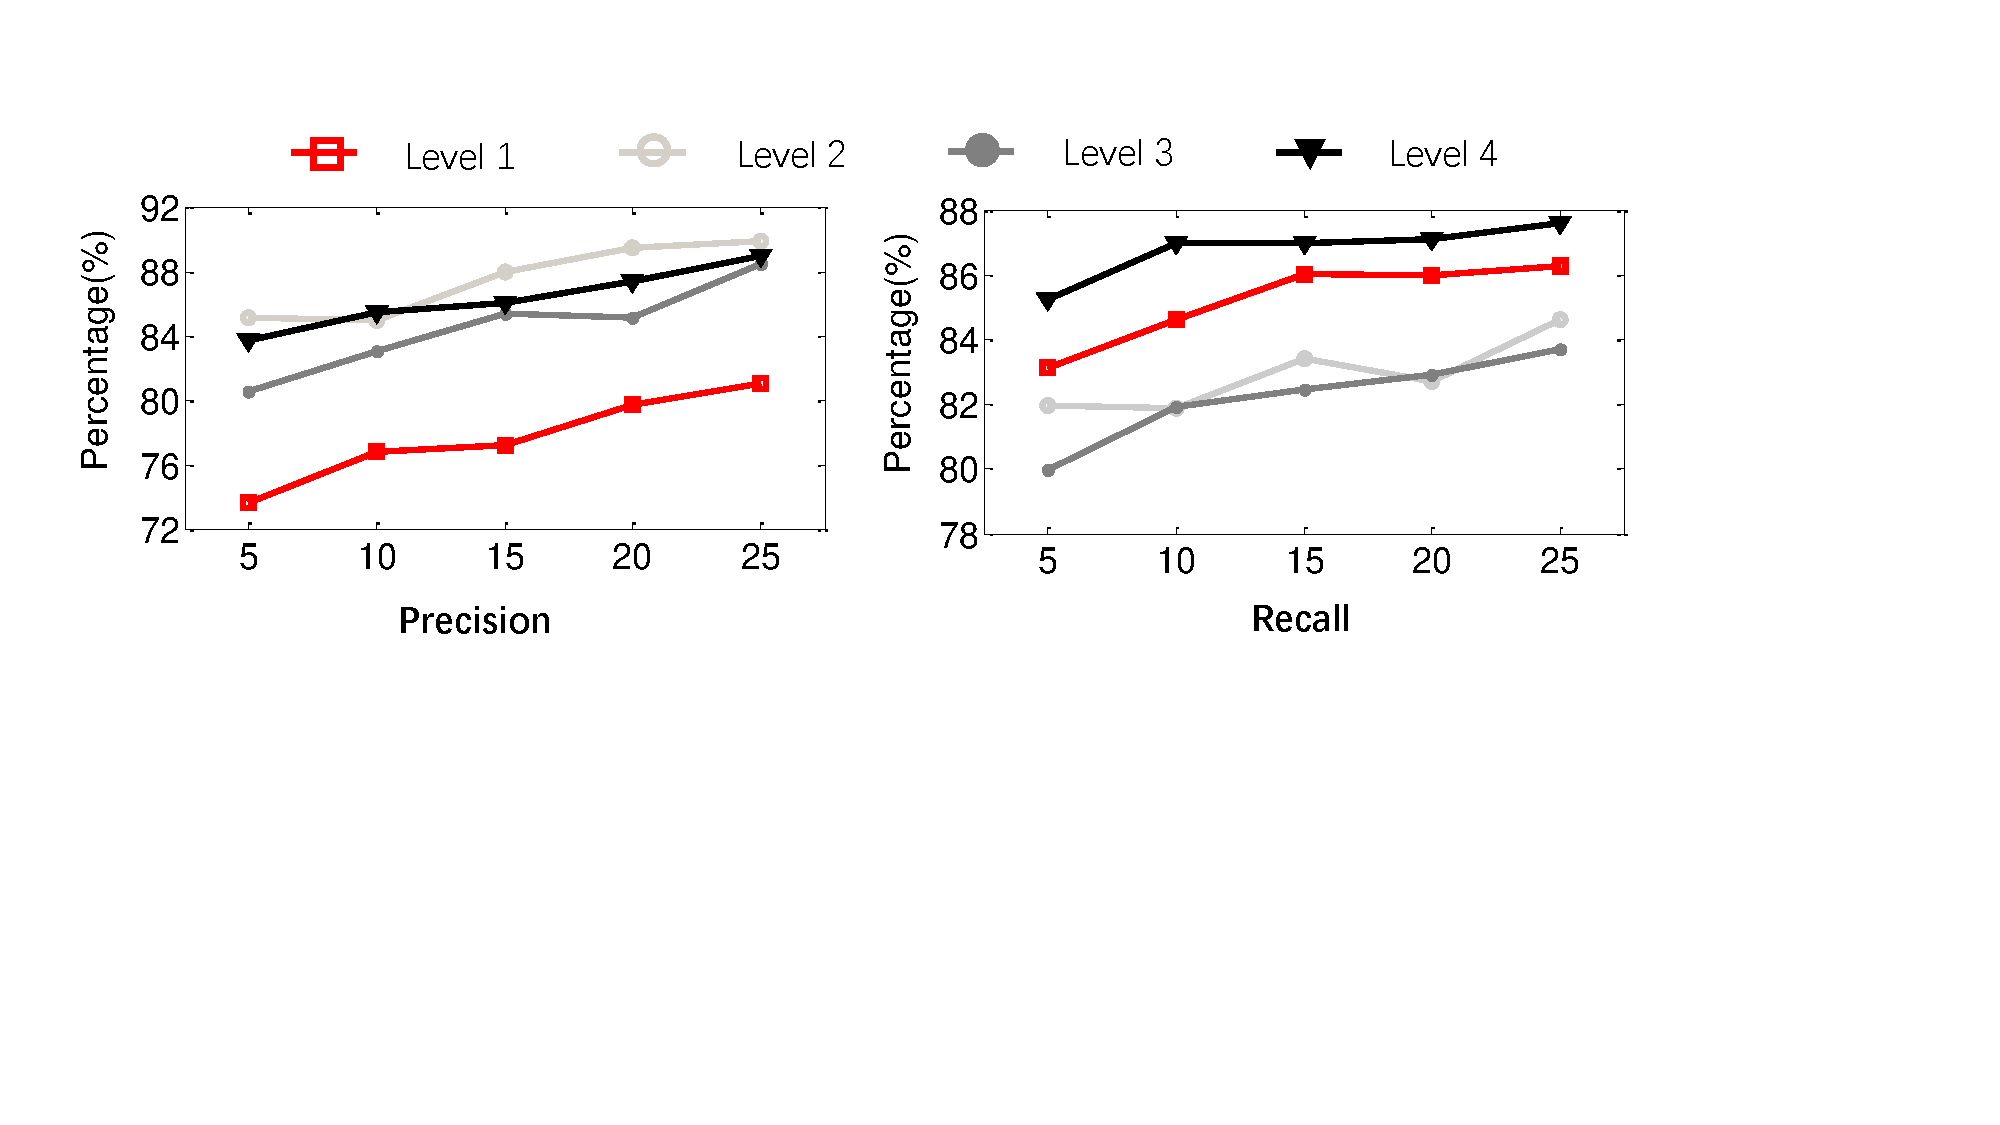
\includegraphics[width=0.9\columnwidth]{./img/performance_under_days.pdf}
\caption{System performance under different training date}
\label{fig:per_under_train_days}
\end{figure}



\paragraph{Evaluation with various prediction duration}

Considering the uncertainties of blood glucose increase while the time passing by, we detail the system performance by differentiating the prediction durations in  Fig.~\ref{fig:per_under_various_pred_days}.
As expected, the system performance shows a decrease trend while the prediction duration leave longer away. It is possible due to the internal relevant factors of blood glucose changed with the time passing by. However, the system performance still can maintain an acceptable level for 30-days prediction.



\begin{figure}[!t]
\centering
\includegraphics[width=0.9\columnwidth]{./img/Performance under prediction
longer.pdf}
\caption{System performance under different prediction duration}
\label{fig:per_under_various_pred_days}
\end{figure}



\subsubsection{Evaluation on Features}

We show the effectiveness of four-dimensional feature in Table ~\ref{Feature_Evaluation}. Clearly, the tracking performance of \sysname improve a lot by adding one feature set into the model.



\begin{table}[]
\small
\centering
\caption{Feature Evaluation}
\label{Feature_Evaluation}
\begin{tabular}{|c|c|c|c|c|c|c|c|c|}
\hline
                                   & \multicolumn{2}{c|}{\textbf{Level 1}}                     & \multicolumn{2}{c|}{\textbf{Level 2}} & \multicolumn{2}{c|}{\textbf{Level 3}}                     & \multicolumn{2}{c|}{\textbf{Level 4}}                     \\ \hline
\textbf{Features}                  & \textbf{Precision} & \multicolumn{1}{l|}{\textbf{Recall}} & \textbf{Precision}  & \textbf{Recall} & \textbf{Precision} & \multicolumn{1}{l|}{\textbf{Recall}} & \textbf{Precision} & \multicolumn{1}{l|}{\textbf{Recall}} \\ \hline
$F_{p}$                            & 43.37$\%$               & 32.82$\%$                                 & 46.03$\%$                & 39.10$\%$            & 51.79$\%$               & 48.95$\%$                                 & 56.30$\%$               & 43.49$\%$                                 \\ \hline
$F_{p}$+$F_{t1}$                   & 51.97$\%$               & 58.11$\%$                                 & 60.42$\%$                & 58.90$\%$            & 63.35$\%$               & 53.59$\%$                                 & 69.82$\%$               & 55.16$\%$                                 \\ \hline
$F_{p}$+$F_{t1}$+$F_{t2}$          & 64.60$\%$               & 73.08$\%$                                 & 69.87$\%$                & 61.23$\%$            & 74.33$\%$               & 67.81$\%$                                 & 76.64$\%$               & 72.32$\%$                                 \\ \hline
$F_{p}$+$F_{t1}$+$F_{t2}$+$F_{t3}$ & 73.62$\%$   & 83.13$\%$                                 & 83.13$\%$               & 83.13$\%$            & 80.55$\%$   & 79.97$\%$
& 83.72$\%$               & 85.23$\%$                                  \\ \hline
\end{tabular}
\end{table}


\subsubsection{Blood glucose level predictions}

Fig.~\ref{fig:pre_gt} compares the predictive results of \sysname and true blood glucose level of a user over one day.






\begin{figure}[!t]
\centering
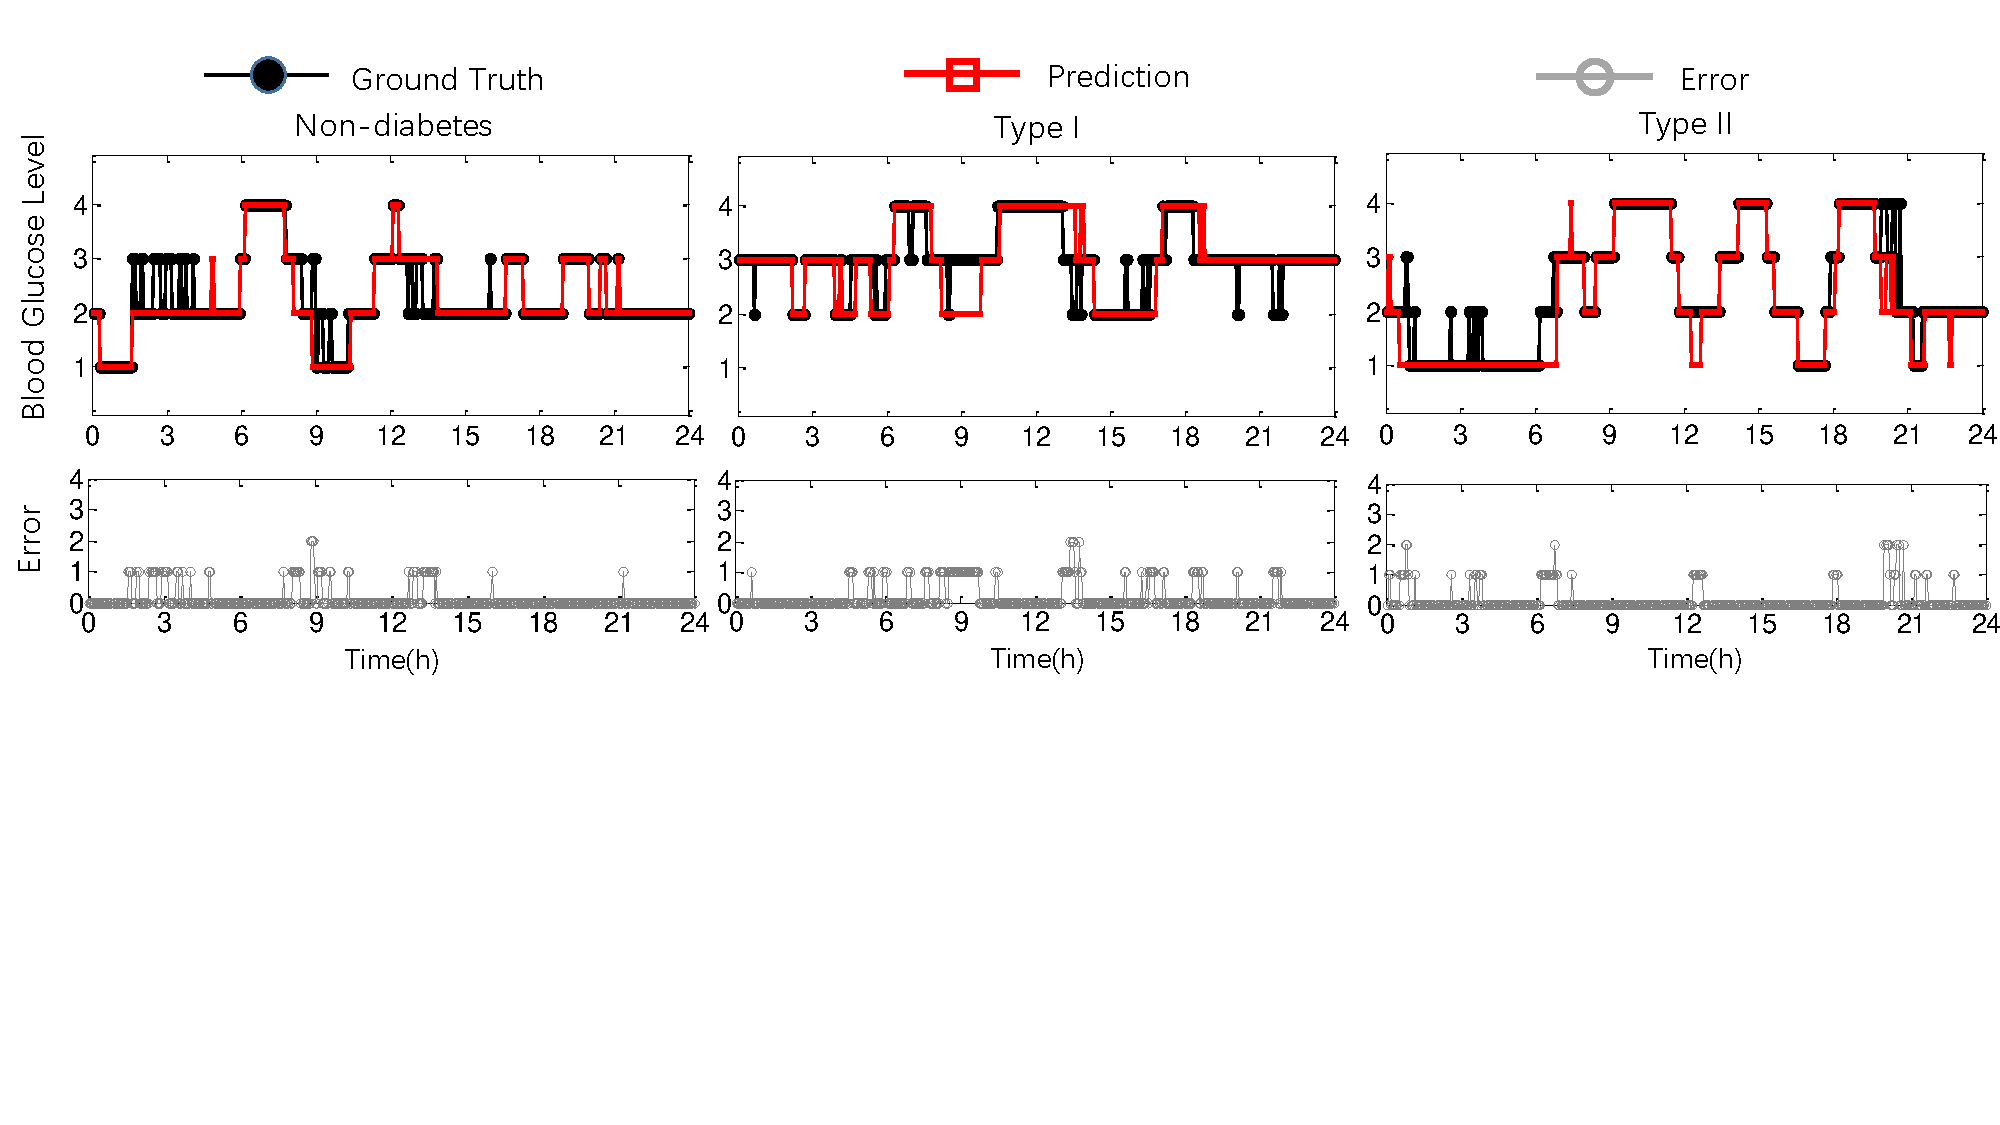
\includegraphics[width=0.5\columnwidth]{./img/pred_vs_gt.pdf}
\caption{The comparison of prediction and the ground truths of one user.}
\label{fig:pre_gt}
\end{figure}


\subsubsection{Model comparison}

We compare \modelname of \sysname over following baselines:

1) Gradient Boosting (GB): GB generates a prediction model by combining many weak classifiers into a stronger classification committee. We use AdaBoost procedure implemented in the fastAdaboost package to combine basic tree classifiers for ensemble learning. We vary the maximum tree depth from 10 to 50 by factors of ten. The number of boosting iterations is varied from 100 to 500 by a step size of 50.

2) Support Vehicle Machine (SVM): SVM bases on the idea of “optimal separating hyperplane” that maximizes the separation margin of two data groups (classes). Due to this construction, it usually generalizes well, and its dual form is a quadratic programing that can be easily incorporated with kernels. We train the Gaussian kernel SVM classifier with the kernlab package, which implements the sequential minimal optimization algorithm. We vary the kernel width from $2^{-5}$ to $2^4$ with a factor of 2. We pick the penalty parameter from the set $\{10^i | i = -3, 0.5, 2\}$. To eliminate scale/location discrepancies among input variables, all features are normalized before being used in the training phase.

3) Hidden Markov model (HMM):

4) Logistic Regression (LR): LR models the posterior distribution of the class labels as a sigmoidal function of linear combinations of features. We use the glmnet package to train LR models with elastic net (combined L1 and L2) regularization. We vary the penalty parameter from 10$^{-3}$ to 10$^2$ with a factor 5. The mixing parameter is varied from 0 (Ridge) to 1 (Lasso) by a step size of 0.1.

5) Random Forest (RF): As another ensemble method, RF combines many simple decision trees together and output the mode of classes for prediction. To avoid correlation among base trees, random set of features are selected in the splitting process when constructing each decision tree. For implementation, we adopt the conditional inference tree algorithm in the Party package. The total number of trees is tuned from 100 to 1000, and the maximum tree depth from 10 to 50. The splitting threshold is also varied from 0.1 to 0.9 with 0.1 intervals for cross validation.

6) Gaussian Processes (GP): Instead of directly parameterizing a latent function for classification, GP models it with a generic Gaussian process. The posterior of the process is updated with training data set, and is “squashed” through a logistic function for classification. We implement GP with the kernlab package, which includes several approximation algorithms for acceleration. We use the radial basis kernel and vary the kernel width from 2$^{-5}$ to 2$^4$ with an incremental factor of 2$^{0.5}$.





